\documentclass{beamer}
\usepackage[orientation=landscape, size=a0, scale=1.4]{beamerposter}
\usepackage[absolute,overlay]{textpos}
\usepackage{multicol}
\usepackage{graphics}
\usepackage{url, enumitem}
\usepackage{amsfonts}
\usepackage{listings}
\usepackage{graphicx}
\usepackage{bm}
\usepackage{tikz}
\usetikzlibrary{fit,positioning}
  \usetheme{CambridgeUS}
    \title[Designator]{Designator}
    \addtobeamertemplate{frametitle}{\vskip0.6ex}{}
\newcommand{\N}{\mathcal{N}}	
\begin{document}

%\begin{block}{\centering \Huge {Title Goes Here}}
%\end{block}
\begin{frame}{\centerline{\Huge Gabriel Doesn't Know How to Refactor Code}}
\begin{textblock}{5}(.15,.85)
\begin{block}{Introduction}
Over the past decade, aesthetics have gained a lot of importance in the decisions companies
make in how they design websites, and user experience is at the core of this trend. One way to
automate part of the creative process of web design is to generate suggestions based on what
popular similar websites contain that the input website does not yet have. Finding "similar
websites," however, can prove to be a daunting task, since diffing a screenshot or even the
color histogram of a given input website against thousands or millions of other websites in a
database is unfeasibly slow. This paper applies Affinity Propagation, an unsupervised clustering
technique, to solve this problem. Once the website database is clustered, the system can place
any input website into a specific cluster. Diffing the input against all websites in a cluster can be
done much faster than within the whole database, and the system will only have to consider
recommendations that are relevant to that specific cluster. 
\end{block}

\begin{block}{Approach}
We implemented a naive recommendation scheme that first clusters all websites, and then
given some incoming website x, first finds the cluster it belongs to and in that cluster finds the
image that is closest to it (which means finding the one with the smallest difference in
histograms). From there, it recommends adding the color that would bring the two images the
closest.
The approach above completely disregards all but the closest sample in the cluster. We wish to
improve it by answering the "ugly duckling" question. Namely if x is our input and Y is a cluster
of websites, what color appears consistently in Y that does not appear in x?
\end{block}

\begin{block}{Graphical Models}
\begin{figure}
\centering
\begin{tikzpicture}
\tikzstyle{main}=[circle, minimum size = 10mm, thick, draw =black!80, node distance = 16mm]
\tikzstyle{connect}=[-latex, thick]
\tikzstyle{box}=[rectangle, draw=black!100]
\node[main, fill = white!100] (Normal) [above] {$\N$ };
\node[main, fill = white!100] (Color) [above=of Normal] {$C$ };
\node[main] (Web) [right=of Color] {$W$};
\node[main,fill={rgb:red,243;green,243;blue,243}] (WebLessColor) [above=of Web, yshift=15mm, xshift=-10mm] {$W_{c}$};
  \path (Normal) edge [connect] (Color)
  	(Web) edge [connect] (Color)
  	(Color) edge [connect] (WebLessColor)
  	(Web) edge [connect] (WebLessColor);
\end{tikzpicture}
\end{figure}
\end{block}


\end{textblock}

\begin{textblock}{5}(5.5, .85)
\begin{block}{Materials And Methods}
Lorem ipsum dolor sit amet, consectetur adipiscing elit, sed do eiusmod tempor incididunt ut labore et dolore magna aliqua. Ut enim ad minim veniam, quis nostrud exercitation ullamco laboris nisi ut aliquip ex ea commodo consequat. Duis aute irure dolor in reprehenderit in voluptate velit esse cillum dolore eu fugiat nulla pariatur. Excepteur sint occaecat cupidatat non proident, sunt in culpa qui officia deserunt mollit anim id est laborum.
\end{block}
\begin{block}{Clustering on K-Means using Band Histograms}
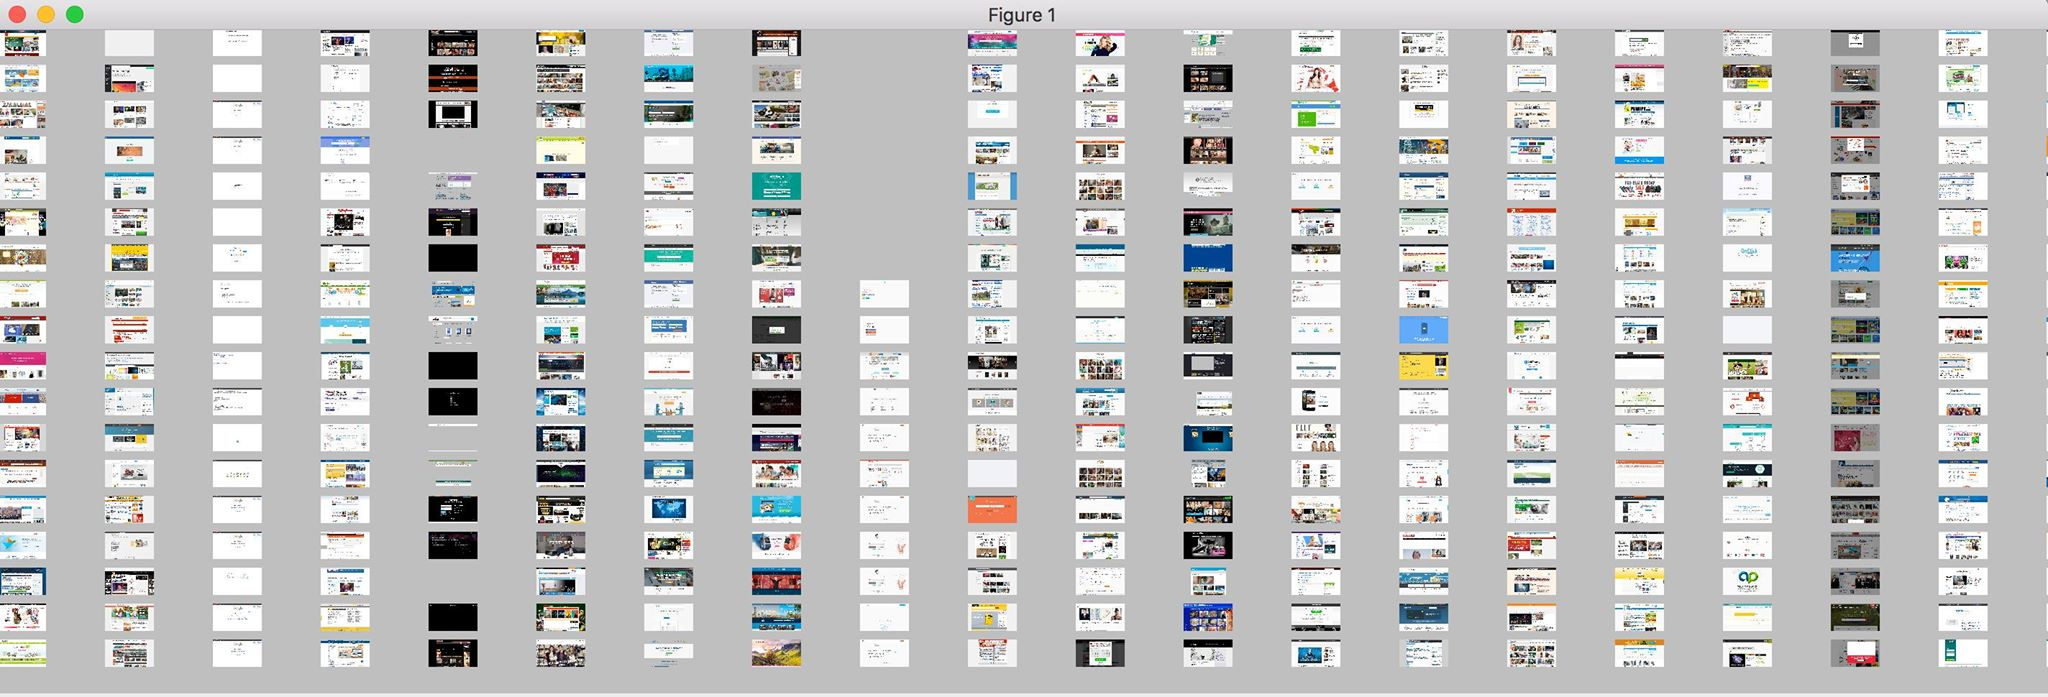
\includegraphics[scale=.5]{histkmeans.png}
\end{block}
\begin{block}{Clustering on K-Means using Images}
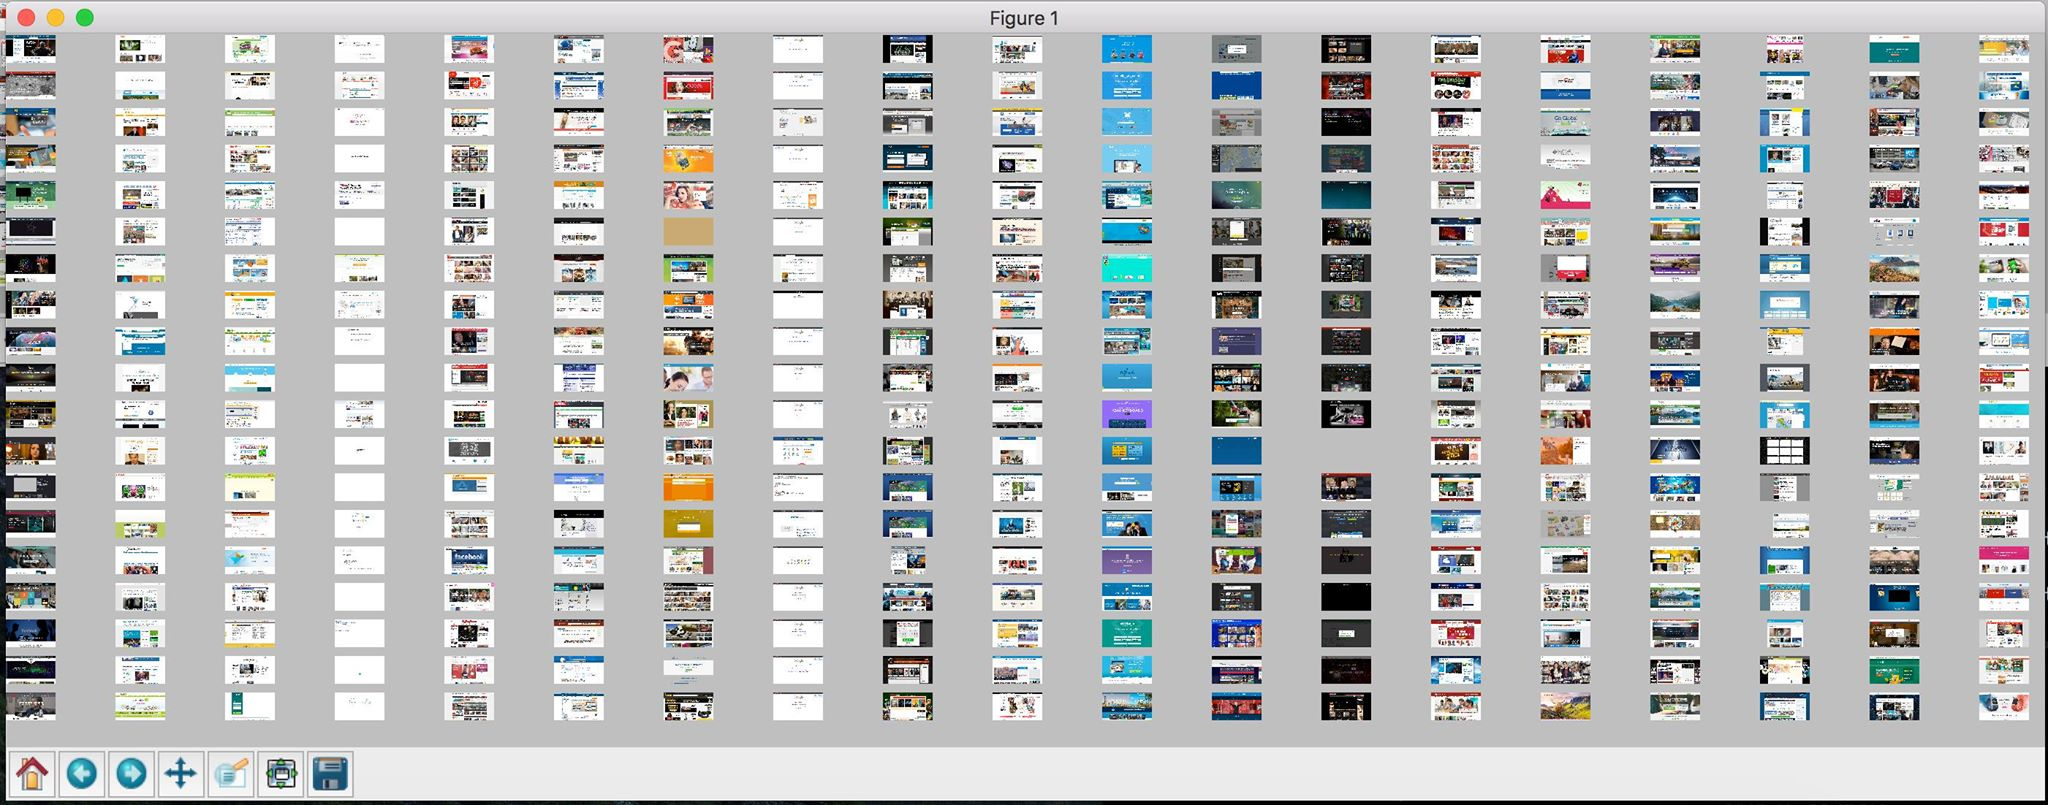
\includegraphics[scale=.5]{imgkmeans.png}
\end{block}
\begin{block}{Clustering on K-Means using Binned Histograms}
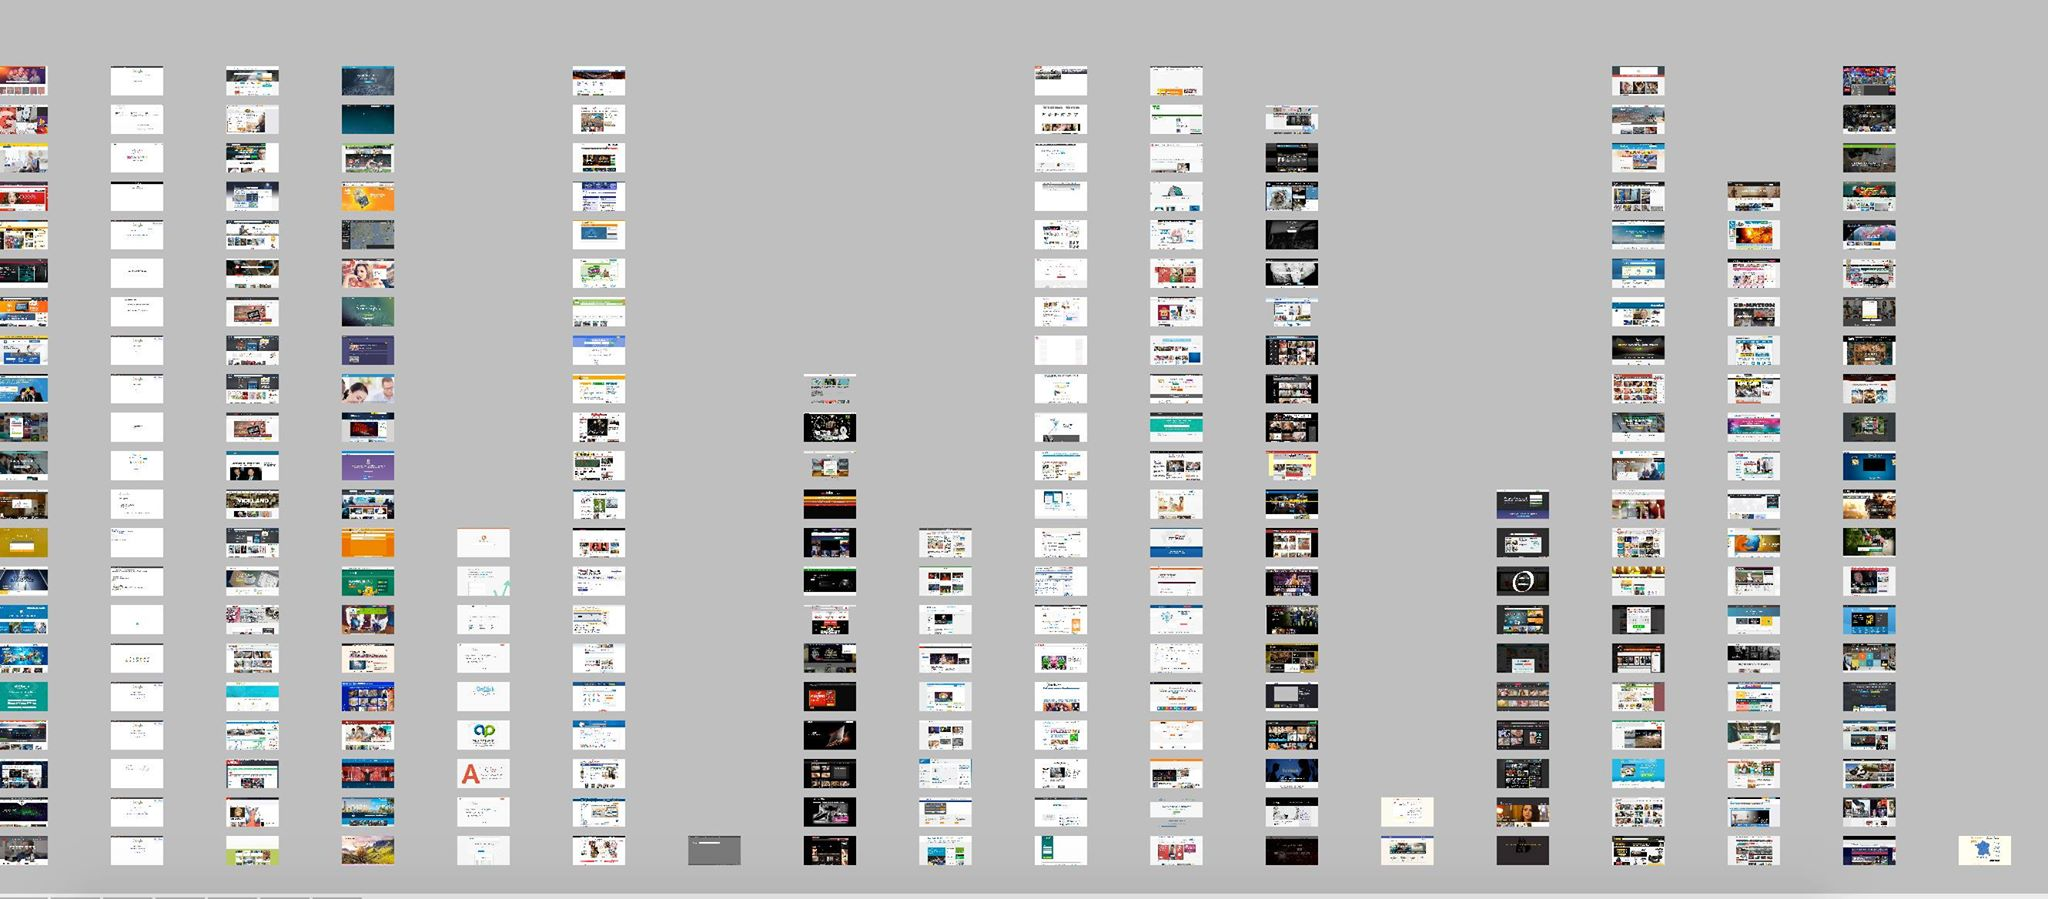
\includegraphics[scale=.5]{binKmeans.jpg}
\end{block}

\end{textblock}
\end{frame}
\end{document}